% ----- Consignes exo 2 ----- %
\begin{td-exo}[Bornes géométriques pour le problème du \textsc{Voyageur de Commerce}]\,\\ % 2 
    On considère le problème du \textsc{Voyageur de Commerce} sur un graphe complet non-orienté formé de \(n\) villes.
    On note \(E\) l'ensemble des arêtes, formé des \(n(n-1)/2\) parties \(\{i,j\}\) de deux éléments distincts de \(\{1,\ldots,n\}\).
    On note \(d_{ij}\) la distance de la ville \(i\) à la ville \(j\).
    On rappelle qu'à un tour, on associe un vecteur \(x\in \bb R^E\) tel que \(x_{ij} = 1\) si l'arête \({i,j}\) appartient au tour et \(x_{ij}=0\) sinon.
    On considère le problème linéaire \(P_1\) (sans contraintes d'intégrité) suivant:
    \begin{equation*}
        (P_1) = 
        \begin{cases}
            \min \sum_{\{i,j\}\in E} d_{ij} x_{ij},\ x\in\bb R^E\\
            \sum_{j:\{i,j\}\in E} x_{ij} = 2,\ \forall i \in \{1,\ldots,n\}\\
            x_{ij} \geq 0,\ \forall \{i,j\} \in E
        \end{cases}
    \end{equation*}
    \begin{enumerate}
        \item Démontrer que la valeur de ce problème minore la valeur du problème du \textsc{Voyageur de Commerce}.
        Si ce problème admet une solution optimale à valeurs dans \(\{0, 1\}\), celle-ci fournit-elle nécessairement un tour optimal?

        \item On propose le minorant suivant, de nature géométrique, de la valeur du problème du \textsc{Voyegeur de Commerce}.
        Nous supposerons que la distance \(d\) provient d'une norme, que pour fixer les idées, nous pourrons supposer être la norme euclidienne dans le plan.
        Autrement dit, chaque ville \(i\) est située en un point \(x_i\in \bb R^2\) de sorte que 
        \begin{equation*}
            d_{ij} = \| x_i - x_j \|
        \end{equation*}
        où \(\|\cdot\|\) désigne la norme euclidienne.
        Donnons-nous un réel \(r_i\geq 0\) pour chaque ville \(i\).
        On dit alors que les disques ouverts
        \begin{equation*}
            D(x_i, r_i) = \left\{
                y \in \bb R^2\ |\ \| y - x_i\| < r_i
            \right\}
        \end{equation*}
        constituent une famille de \textit{zones de controle} s'ils sont deux à deux disjoints.
        Montrer que si les \(r_i\) sont les rayons des disques d'une famille de zones de controle alors la valeur d'un tour est minorée par \(\sum_{1 \leq i \leq n} 2r_i\).
        En déduire que la zone valeur du problème du \textsc{Voyageur de Commerce} est minorée par la valeur du problème suivant:
        \begin{equation*}
            D_1 = 
            \begin{cases}
                \max \sum_{i=1}^n 2r_i,\ r_i\in\bb R^n\\
                r_i + r_j \leq d_{ij},\ \forall {i,j}\in E\\
                r_i\geq 0,\ \forall i \in \{1,\ldots n\}
            \end{cases}
        \end{equation*}

        \item Montrer que si un tour est tel qu'il existe une famille de zones de controle telles que 
        \begin{equation*}
            d_{ij} = r_i + r_j
        \end{equation*}
        pour toute arête \(\{i,j\}\) du tour alors ce tour est optimal.

        \item Expliciter le problème dual du problème \(P_1\) et le comparer au programme \(D_1\).
        Retrouver ainsi la borne précédente faisant intervenir les zones de controle.

        \item Que pensez-vous de la qualité des bornes précédentes pour l'instance donnée par la figure 1 répartie en deux groupes distants?

        \ffigbox[\FBwidth]{%
\caption{\centering Le pire des cas pour les zones de controle}\label{fig:dm1_ex02_f1}
}{
    \fbox{
        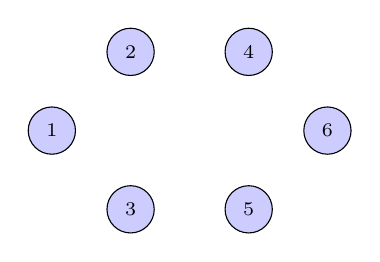
\begin{tikzpicture}[scale=1, main node/.style={circle, draw, fill=blue!20, inner sep=1pt, font=\scriptsize, minimum size=6mm, text=black}]
            % les sommets initiaux
            \node[main node] (1) at (0,0) {\(1\)};
            \node[main node] (2) at (1,1) {\(2\)};
            \node[main node] (3) at (1,-1) {\(3\)};
            
            \node[main node] (4) at (2.5,1) {\(4\)};
            \node[main node] (5) at (2.5,-1) {\(5\)};
            \node[main node] (6) at (3.5,0) {\(6\)};

        \end{tikzpicture}
    }
}

        Afin d'améliorer la borne obtenue à l'aide des zones de controle nous introduisons maintenant la notion suivante:

        Etant donné un sous-ensemble non-vide \(V\) de villes ainsi qu'une famille de zones de controle, nous appelons \defemph{douve} de largeur \(\delta\) centrée en \(V\) la région:
        \begin{equation*}
            D = \left\{
                y\in \bb R^2\ |\ \exists x_i\in V, \|y-x_i\| \leq r_i + \delta
            \right\}
        \end{equation*}
        On notera \(\ol V\) le complémentaire de \(V\) dans l'ensemble des villes.

        \item Montrer que si deux douves centrées respectivement en \(V\) et en \(\ol V\) et de largeurs respectives \(\delta\) et \(\ol\delta\) ne s'interceptent pas alors la somme
        \begin{equation*}
            \sum_{i=1}^n 2r_i + 2\delta + 2\ol\delta
        \end{equation*}
        minore la valeur du problème du \textsc{Voyageur de Commerce}.

        \item Considérons maintenant le problème \(P_2\) obtenu en rajoutant à \(P_1\) une unique contrainte de sous-tour:
        \begin{equation*}
            \sum_{\{i,j\}\in E,i\in V,j\in\ol V} x_{ij} \geq 2
        \end{equation*}
        Expliciter le dual du problème \(P_2\).
        Montrer que toute borne obtenue à l'aide de douves peut aussi être obtenue à l'aide d'une contrainte de sous-tour.

        \item On considère l'instance donnée par la figure 2. 
        
        \ffigbox[\FBwidth]{%
\caption{\centering Figure temporaire a remplacer par une grille}\label{fig:dm1_ex02_f2}
}{
    \fbox{
        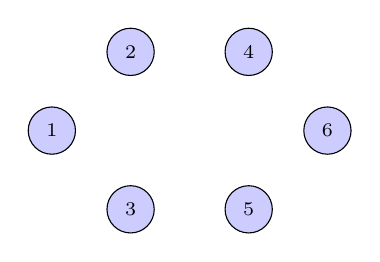
\begin{tikzpicture}[scale=1, main node/.style={circle, draw, fill=blue!20, inner sep=1pt, font=\scriptsize, minimum size=6mm, text=black}]
            % les sommets initiaux
            \node[main node] (1) at (0,0) {\(1\)};
            \node[main node] (2) at (1,1) {\(2\)};
            \node[main node] (3) at (1,-1) {\(3\)};
            
            \node[main node] (4) at (2.5,1) {\(4\)};
            \node[main node] (5) at (2.5,-1) {\(5\)};
            \node[main node] (6) at (3.5,0) {\(6\)};

        \end{tikzpicture}
    }
}
        On prend la distance \(L_1\) et non la distance euclidienne.
        Les notions de disques, de zones de controle et de douves s'entendent alors au sens de cette distance.
        Montrer directement à l'aide d'une borne en faisant intervenir des douves que la longueur minimale d'un tour est de 14.
    \end{enumerate}
\end{td-exo}

% ----- Solutions exo 2 ----- %
\iftoggle{showsolutions}{ 
	\begin{td-sol}[]\ % 2
		\begin{enumerate}
            \item Commencons par expliciter l'ensemble des solutions des deux problèmes.

            Pour le problème du \textsc{Voyageur de Commerce} on a:
            \begin{equation*}
                S_{TSP} = \left\{
                    x \in {\{0,1\}}^E\ |\ \sum_{j\colon \{i, j\}\in E} x_{ij} = 2 \ \forall i\text{ et les aretes forment un seul cycle}
                \right\}
            \end{equation*}
            Alors que pour \(P_1\) on a:
            \begin{equation*}
                S_{P_1} = \left\{
                    x \in {\bb R}^E_{+}\ |\ \sum_{j\colon \{i, j\}\in E} x_{ij} = 2 \ \forall i
                \right\}
            \end{equation*}
            Cela montre clairement que 
            \begin{equation*}
                S_{TSP} \subseteq S_{P_1}
            \end{equation*}
            Alors, si on considère la fonction \(f\) suivante:
            \begin{equation*}
                f(x) = \sum_{\left\{i, j\right\}\in E} d_{ij} x_{ij}
            \end{equation*}
            on a bien
            \begin{equation*}
                \underset{x\in S_{P_1}}\min f(x) \leq \underset{x\in S_{TSP}}\min f(x)
            \end{equation*}
            et donc les solutions au problème \(P_1\) minorent les solutions du \textsc{Voyageur de Commerce}.

            De plus, les solutions de \(P_1\) ne sont pas forcément admissibles pour le \textsc{Voyageur de Commerce}.
            Prenons l'exemple suivant avec le graphe \(G\) de la figure~\ref{fig:dm1_ex02_f3} ci-dessous:

            \vspace{9px}
            \ffigbox[\FBwidth]{%
\caption{\centering Le pire des cas pour les zones de controle}\label{fig:dm1_ex02_f1}
}{
    \fbox{
        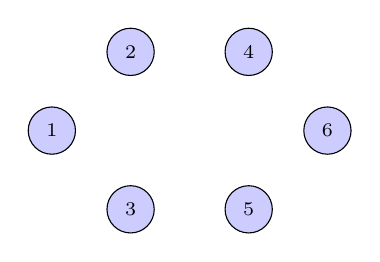
\begin{tikzpicture}[scale=1, main node/.style={circle, draw, fill=blue!20, inner sep=1pt, font=\scriptsize, minimum size=6mm, text=black}]
            % les sommets initiaux
            \node[main node] (1) at (0,0) {\(1\)};
            \node[main node] (2) at (1,1) {\(2\)};
            \node[main node] (3) at (1,-1) {\(3\)};
            
            \node[main node] (4) at (2.5,1) {\(4\)};
            \node[main node] (5) at (2.5,-1) {\(5\)};
            \node[main node] (6) at (3.5,0) {\(6\)};

        \end{tikzpicture}
    }
}

            On peut voir que la solution au problème \(P_1\) sur \(G\) où la distance entre les sommets est, par simplicité, la distance euclidienne donne
            \begin{equation*}
                S_0 = \left\{
                    \{a, b\}, \{b, c\}, \{c, a\}, \{1, 2\}, \{2, 3\}, \{3, 1\}
                \right\}
            \end{equation*}
            où les arêtes dans \(S_0\) ont poids \(1\) dans la solution et les autres ont poids 0.

            Cette solution respecte bien toutes les contraintes de \(P_1\) mais correspond à deux cycles disjoints et n'est donc pas solution du \textsc{Voyageur de Commerce}.
            Ainsi une solution de \(P_1\), même si elle est dans \(\{0, 1\}\) ne fournit pas forcément un tour optimal pour le problème du \textsc{Voyageur de Commerce}.

            \item Si l'ensemble des \(r_i\) forment une famille de zones de controles alors ils sont deux à deux disjoints.
            En particulier, pour tout \(\{i,j\}\in E\), on a
            \begin{equation*}\label{eq:dm1_ex02_e1}
                r_i + r_j \leq d_{ij}
            \end{equation*}
            Sinon, les deux disques respectivement centrés en \(i\) et \(j\) se croiseraient car ils dépassent la distance entre \(i\) et \(j\).
            De plus, une solution au problème du \textsc{Voyageur de Commerce} passe forcément par chaque sommet.
            En particulier, si on considère les disques de rayon \(r_i\) de chaque sommet et une solution \(x_0,x_1,\ldots,x_k,x_0\) au problème du \textsc{Voyageur de Commerce}, on a:
            \begin{equation*}
                d_{x_i x_{i+1}} \geq r_i + r_{i+1}
            \end{equation*}
            En effet, une simple représentation géométrique de cela consisterait à tracer les deux disques respectivement centrés en \(x_i\) et \(x_{i+1}\) de rayons respectifs \(r_i\) et \(r_{i+1}\).
            Alors, la droite qui passe par \(x_i\) et \(x_{i+1}\) passe forcément par le disque \(D(x_i, r_i)\) car il faut \og{}sortir de ce disque{} pour atteindre \(x_{i+1}\) (car les disques ne contiennent pas d'autres sommets par~\eqref{eq:dm1_ex02_e1}).
            Il en va de même pour le disque en \(D(x_{i+1}, r_{i+1})\).
            Alors on a bien
            \begin{equation*}
                d_{x_i x_{i+1}} \geq r_i + r_{i+1}
            \end{equation*}
            et il en suit
            \begin{equation*}
                \sum_{\{i, j\}\in S} d_{ij} \geq \sum_{i=1}^n 2 r_i
            \end{equation*}
            car chaque sommet apparait deux fois dans la somme des distances dans la solution (il faut \og{}rentrer\fg{} dans le sommet puis en ressortir). D'où
            \begin{equation*}
                D_1 = 
                \begin{cases}
                    \max \sum_{i=1}^n 2r_i,\ r_i\in\bb R^n\\
                    r_i + r_j \leq d_{ij},\ \forall {i,j}\in E\\
                    r_i\geq 0,\ \forall i \in \{1,\ldots n\}
                \end{cases}
            \end{equation*}
            comme borne inférieure aux solutions du problème.

            \item Soit \(S\) une solution telle que
            \begin{equation*}
                d_{ij} = r_i + r_j.
            \end{equation*}
            On sait par la question précédente que 
            \begin{equation*}
                \sum_{i=1}^n 2r_i
            \end{equation*}
            est un minorant de toute solution.
            De plus, 
            \begin{equation*}
                \sum_{\{i, j\}\in S} d_{ij} = \sum_{\{i, j\}\in S} (r_i + r_j)
            \end{equation*}
            par hypothèse.
            Cette solution étant un cycle hamiltonien, on sait que chaque sommet apparait exactement 2 fois dans la somme des distances, alors on a
            \begin{equation*}
                \sum_{\{i, j\}\in S} (r_i + r_j) = \sum_{i=1}^n 2r_i.
            \end{equation*}
            Soit \(S\) atteint la borne inférieure des solutions à ce problème, donc elle est optimale.

            \item Le problème \(P_1\) a une variable par arête (non orientée) et il y a \(n\) sommets donc \(\frac{n(n-1)}2\) variables.
            On a une contrainte par sommet et \(n\) sommets donc \(n\) contraintes.
            Le dual aura donc \(n\) variables et \(\frac{n(n-1)}2\) contraintes (autrement dit, autant de contraintes que d'arêtes).

            Cela donne:
            \begin{equation*}
                \mathsf{Dual}(P_1) = 
                \begin{cases}
                    \max \sum_{i=1}^n 2y_i\\
                    y_i + y_j \leq d_{ij},\ \forall \{i,j\}\in E
                \end{cases}
            \end{equation*}
            Cela correspond bien au bon nombre de variables et de contraintes.
            Il n'y a qu'une seule différence avec le programme \(D_1\), on n'a pas de contraintes sur le signe de \(y\).
            Si on contraint le dual aux valeurs positives en \(y\) alors on retrouve bien le programme \(D_1\) et la borne précédente.
            De plus, visuellement, si on considère qu'un \(r_i\) négatif ne correspond qu'à agrandir le rayon du disque dans l'autre sens, cela ne change rien aux solutions ni aux disques utilisés (ce n'est que visuel, plus formellement si on utilise \(|r_i|\) au lieu de juste \(r_i\) alors on a bien les mêmes propriétés sans contraindre le signe de \(r_i\)).

            \item On peut facilement remarquer que lorsque nos sommets sont proches, ou du moins à des distances similaires, l'utilisation de disques permet de bien séparer les sommets tout en mesurant la distance entre ceux-ci avec peu de perte.
            Dans le cas de la figure~\ref{fig:dm1_ex02_f1} on comprend que si les sommets \(A = \{1,2,3\}\) sont très proches entre eux, les sommets \(B = \{4, 5, 6\}\) aussi mais ces deux groupes distants l'un de l'autre, alors les sommets au sein de \(A\) (et de \(B\)) vont fortement restreindre la taille des disques des autres sommets au sein du même groupe.
            Cela n'a pas forcement d'effet negatif au sein même de \(A\) mais donne une borne mauvaise sur la distance totale car elle neglige completement l'ecart entre ces deux groupes (qui pourtant contribue pour la majorité du poids d'une solution).

            La notion de douve introduite pour la suite de l'exercice permet de parfaitement répondre à ce problème en regroupant ainsi les zones de controle par sous-famille locale, en découpant l'espace en régions en quelque sorte.
            Cela permettrait alors, dans le cas de la figure~\ref{fig:dm1_ex02_f1} par exemple de mesurer l'ecart entre les groupes \(A\) et \(B\) avec les douves tout en conservant les ecarts entre les villes internes à ces groupes grace aux zones de controle.

            Une représentation de ces concepts est donnée dans la figure~\ref{fig:dm1_ex02_f4} ci-dessous:

            \ffigbox[\FBwidth]{%
\caption{\centering Illustration des zones de contrôle sur la figure~\ref{fig:dm1_ex02_f1}}\label{fig:dm1_ex02_f4}
}{
    \fbox{
        \begin{tikzpicture}[scale=1, main node/.style={circle, draw, fill=blue!20, inner sep=1pt, font=\scriptsize, minimum size=6mm, text=black}]
            % gonna need these for the annoying circles later
            \def\ra{1}      % original control radius
            \def\rb{0.56}      % original control radius
            \def\delta{0.5}   % douve thickness
            \def\Ra{\ra+\delta} % expanded radius
            \def\Rb{\rb+\delta} % expanded radius
            % thick line = 0.8pt -> half = 0.4pt = 0.014058cm
            \def\lwh{0.014058}
            \def\Rta{\Ra-\lwh}
            \def\Rtb{\Rb-\lwh}

            % nodes
            \node[main node] (1) at (-0.2,0) {1};
            \node[main node] (2) at (1,1) {2};
            \node[main node] (3) at (1,-1) {3};
            
            \node[main node] (4) at (4,1) {4};
            \node[main node] (5) at (4,-1) {5};
            \node[main node] (6) at (5.2,0) {6};

            % small circles for group 1-2-3
            \draw[red, thick, fill=red!20] (1) circle (\rb);
            \draw[red, thick, fill=red!20] (2) circle (\ra);
            \draw[red, thick, fill=red!20] (3) circle (\ra);

            % small circles for group 4-5-6
            \draw[red, thick, fill=red!20] (4) circle (\ra);
            \draw[red, thick, fill=red!20] (5) circle (\ra);
            \draw[red, thick, fill=red!20] (6) circle (\rb);
            
            \node[main node] (1bis) at (-0.2,0) {\(1\)};
            \node[main node] (2bis) at (1,1) {\(2\)};
            \node[main node] (3bis) at (1,-1) {\(3\)};
            
            \node[main node] (4bis) at (4,1) {\(4\)};
            \node[main node] (5bis) at (4,-1) {\(5\)};
            \node[main node] (6bis) at (5.2,0) {\(6\)};

            % Douves
            % draw outline (with overlaps) first then fill
            \begin{scope}[on background layer]
                \foreach \v in {2,3,4,5} {
                    \draw[fill=green!30, thick, draw=green] (\v) circle (\Ra);
                }
                \foreach \v in {1,6} {
                    \draw[fill=green!30, thick, draw=green] (\v) circle (\Rb);
                }
                \foreach \v in {2,3,4,5} {
                    \fill[green!30] (\v) circle (\Rta);
                }
                \foreach \v in {1,6} {
                    \fill[green!30] (\v) circle (\Rtb);
                }
            \end{scope}

            % ------------------------
            % Legend to the side
            % ------------------------
            \begin{scope}[shift={(7,2)}, font=\scriptsize]
                \node[draw=red, thick, minimum width=0.35cm, minimum height=0.35cm, fill=red!20] (leg1) {};
                \node[right=0.25cm of leg1, anchor=west] {Zones de contrôle};

                \node[draw=green, thick, minimum width=0.35cm, minimum height=0.35cm, below=0.3cm of leg1, fill=green!30] (leg2) {};
                \node[right=0.25cm of leg2, anchor=west] {Douves};
            \end{scope}

        \end{tikzpicture}
    }
}


            où les zones rouges représentent des zones de controle de taille maximale locale (si on se restreint à la partie de gauche ou à la partie de droite ces rayons sont maximaux).
            Les zones vertes représentent les douves maximales.

            On peut alors voir l'interet visuel de ces différents objets: les zones de controle permettent de bien mesurer la distance locale au sein d'un groupe et les douves permettent de mesurer la distance entre ces groupes.

            \item Cela correspond à la même preuve que sur les zones de controle plus tot.
            Si une des douves est vide (par exemple si son complémentaire contient tout le monde, ce qui n'est pas exclu) alors il n'y a aucun intérêt à utiliser des douves et \(\delta=0\) convient, ce qui donne bien la minoration trouvée précédemment:
            \begin{equation*}
                \sum_{\{i, j\}\in S} d_{ij} \geq \sum_{i=1}^n 2 r_i
            \end{equation*}
            Sinon, chaque douve contient au moins un sommet.
            Alors, un cycle hamiltonien doit forcément passer par ce sommet deux fois et, comme précédemment, doit donc traverser la douve une fois pour rentrer et une fois pour sortir de ce sommet.
            
            On en conclut alors que pour passer d'un sommet de \(V\) au sommet le plus proche dans \(V'\) il faut passer par les deux douves une première fois, puis une autre au retour.
            En y ajoutant les déplacements à l'intérieur même de ces douves on obtient bien
            \begin{equation*}
                \sum_{\{i, j\}\in S} d_{ij} \geq \sum_{i=1} 2 r_i + 2\delta + 2 \ol\delta
            \end{equation*}
        \end{enumerate}
	\end{td-sol}
}{}